\documentclass{template/socthesis}

\usepackage{subcaption}
\usepackage{amsmath}
\usepackage{enumitem}

\addbibresource{text.bib}

\titlecz{Postav si svého prvního robota}
\titleen{Build your first robot}
\author{Tomas Vavrinec}
\field{10}
\school{Střední průmyslová škola a Vyšší odborná škola Brno, Sokolská}
\mentor{Mgr.Miroslav Burda}
\mentorstatement{doc. PhDr. Jany Novákové, Ph.D.}

% Změňte, pokud se liší
%\region{Jihomoravský}
%\placefooter{Brno 2017}

\begin{document}

\maketitle

\makecopyrightstatement{V~Brně}

\makethanks{Děkuji svému školitely Mgr. Miroslavu Burdovi za obětavou pomoc, podnětné připomínky a nekonečnou trpělivost, kterou mi během práce poskytoval.}

\pagestyle{empty}

\section*{Anotace}
Tato práce se zabývá návrhem několika robotických zařízení. Jejich použití při výuce dětí v zájmovém vzdělávání a školní výuce předmětů automatizace a elektrotechniky.
Cílem je především vyvinout vhodné vzdělávací pomůcku, která bude schopná řídit například i soutěžní roboty, nebo výrobní linky.


\subsection*{Klíčová slova}
robot; vyuka robotiky; řídící deska; esp32

\vspace{20mm}

\section*{Annotation}


\subsection*{Keywords}

\newpage
\pagestyle{plain}

\tableofcontents % vysází obsah

%%% Začátek práce
\setcounter{figure}{0}
\setcounter{table}{0}
\newpage

\chapter*{Úvod}
\addcontentsline{toc}{chapter}{Úvod} % přidá položku úvod do obsahu
Projekt má za cíl vytvořit pomůcky pro seznámení s robotikou pro studenty nejen technických oborů případně pro zájemce o studium tohoto oboru. Důvodem k práci byly především nedostatky a velká cena konkurenčních systému. Rozhodl jsem se tedy vyvinout takový systém který by plně vyhovoval účelu a zároveň by nebyl zbytečně drahý.

\section{SchoolBot}
Robot je primárně navržen pro volnočasový vzdělávací kurz robotiky pořádaný na naší škole a je určen pro začátečníky, jako takový dává účastníkům možnosti, které má prakticky každý soutěžní robot, konkrétně pohon, pro pohyb na hřišti a klepeta pro manipulaci s herními prvky.

%\section{BlackBox}
%BlackBox je elektronicky ovládaný trezor, který je s vhodnou úpravou schopen i jezdit na vlastních kolech. Pro začátečníky má i čistě mechanickou variantu bez elektroniky, ta však muže sloužit jen jako trezor a nemá ostatní možnosti které má až elektronická varianta. Elektronická varianta má rozmanité senzory, díky kterým muže nabývat různých podob od trezor po hodiny.


\newpage

\chapter{Proč vytvářet vlastní roboty?}
Proč vlastně vytvářet vlastní elektroniku i mechaniku, když je na trhu tolik různých robotu a vozítek? Konkurenční roboti, kteří se běžně prodávají, jsou totiž většinou velmi drazí a často nemají ani moc možností. Například známé LEGO Mindstorms, u kterého se cena základní sady pohybuje nad sedmi tisíci korunami [], je vzhledem ke svým možnostem ohromně předražené.
 
Při vytváření pokročilejších aplikací potřebuje tvůrce znalost technických specifikací robota a jeho vnitřního fungování. U většiny komerčních robotu však není kompletní technická dokumentace volně dostupná.

\section{Konkurence}

\subsection{LEGO Mindstorms EV3}
LEGO Mindstorms je známé svou jednoduchostí. Základní roboti se s touto sadou dají sestavit velmi rychle, což poskytuje hlavně začátečníkům motivaci, neboť již s poměrně malým úsilím sestaví něco, co na první pohled funguje. Dílky lEGa však nejsou moc pevné a konstrukce z nich postavená jich tedy vyžaduje velké množství, aby byla obstojně tuhá. To se samozřejmě dá jednoduše vyřešit, tím že si člověk udělá konstrukci z jiného materiálu. 
Možnosti robota se z velké části odvíjí od senzoriky. Lego trpí na nedostatek senzoru. Nejen, že v základní sadě je, krom tlačítka, od každého sensory jen jeden kus. Ale ani kostka, řídící centrum lega, nedokáže číst víc než čtyři senzory naráz. Je pravda že lego má možnost spojovat několik kostek dohromady, to však samozřejmě vyžaduje mít jich víc což je při ceně lega poměrně drahé.
Lego má své vlastní programovací prostředí, které je většinou pro začátečníky dobré. Jakmile však člověk chce vytvářet vetší program, prostředí velmi rychle ztratí užitečnost. Vetší programy jsou v grafickém prostředí velmi nepřehledné. Navíc prostředí lega může být u větších programů nestabilní. Existují však i prostředí ze kterých se dá lego programovat textově, například v jazyku C++, což je u složitějších programu přehlednější a také méně náročné pro počítač.

\subsection{Mbot}
Mbot je oproti legu daleko levnější (cena se pohybuje kolem osmnácti set korun za kus) ale trpí stejným, nebo i větším, nedostatkem sensoru. Co se konstrukce týče, problémy s pevností u Mbota není ale zase se nedá snadno upravit. Konstrukce je totiž hliníková, což je v pořádku, pokud není potřeba konstrukci výrazně upravovat. Robota je ale většinou třeba přizpůsobit konkrétnímu užití, ze zkušenosti se nejvíce osvědčilo dřevo, které se dá jednoduše upravovat bez větší námahy a zároveň není problém z něj udělat dostatečně tuhou konstrukci. Hliník se však tak lehce ručně upravovat nedá.
Mbot je založen na procesoru ATmega328 což je stejný procesor jaký se používá i u velice známého arduina. To znamená že některé programy, které jsou napsané pro arduino je možné spustit i zde.

\subsection{Edison}
Edison je velmi podobný legu a mí i podobné problémy. Opět nedisponuje velkým počtem senzoru ale oproti legu je daleko levnější. Stejně jako lego má i Edison vlastní grafické programovací prostředí, bohužel jsem jej nikdy nepoužíval, ale vypadá velmi podobně jako prostředí lega. Myslím si proto, že stejně jako prostředí lega bude i toto velice dobré na malé prográmky pro děti, ale nevhodné pro obsáhlé programy.
Všechny senzory má Edison uvnitř sebe a nedají se proto dovést na místo kde je uživatel nejvíc potřebuje. Uživatel se proto musí přizpůsobit rozložení senzoru na řídící jednotce, stejně tak se nedá vyvést ani nic jiného. Jediné, co se dá, je vyměňovat kola (například za nějaké ozubení) a pomocí toho si pak dovést náhon z motoru na potřebné místo.

\subsection{OZOBOT}
Ozobot je miny robot, z toho vyplývají jeho největší výhody i nevýhody. Například pochopitelně není dělaný na to, aby cokoli vozil nebo jakkoliv stěhoval. Téměř se nedá upravovat, na to ale opět není dělaný jeho účel je především jezdit po čáře a vykonávat příkazy na ní zapsané pomocí barevných vzoru. Přes to že se novější verze dají i programovat, jejich funkce jsou pořád mířené do velké míry právě na čáru a barevné příkazy na ní.

\subsection{Asuro}
Asuro je robot postavený kolem základní desky. Jedná se o stavebnici, ale přesto nemá ani jednoduché pomůcky pro možnost přesné stavby. Asuro má mezi koly a motorem převodovku která se ukládá do jakýchsi ložisek které se bez jakéhokoli za pozicování napájí na plochu desky. Výsledkem je téměř nemožnost uložit kola převodovky přesně.

\subsection{Microbit}
Microbit je především řídící deska se senzory a výstupními ledkami. Není to primárně vozítko, přesto že existují konstrukce, které jsou určené právě pro řízení microbitem. Taková konstrukce však muže využívat pouze serva nebo musí mýt vlastní řízení motoru. Microbit totiž motory řídit nedokáže sám, dokáže řídit jen serva, která si řízení řeší sama. Toto však není velký problém, protože existuje více různých konstrukcí, které právě toto řeší. Microbit má překvapivě docela dost senzoru přímo na základní destičce. Podle mích informací kompas, který je přímo na desce téměř nefunguje ale vzhledem k tomu, co všechno na sobě malá destička Microbit má to není až taková tragédie. Kompas je stejně často potřebné dostat co nejdál od zbytku robota, kvůli všemožnému rušení, takže by so i tak dost možná používal jako externí součástka.
Microbit má zároveň matici ledek na které si uživatel muže zobrazovat co se mu zlíbí a zároveň se jiny dá i měřit světelnost okolí. Používání led diod jako fotodiod sice není tak přesné nicméně to jde a je to velice zajímavé řešení.

\subsection{Shrnutí}
Komerční systémy jsou většinou velmi drahé, nemají zrovna nadbytek senzoru, mívají měkkou nebo obtížně upravitelnou konstrukci a také nemají moc veky výkonu ani přesnost pohonu.
Možná si říkáte proč mi záleží na tom aby robot pro začátečníky mel všechny tyto možnosti. Vždyť člověku, co nikdy robota nestavěl by to mělo být skoro jedno. Ano, vlastně by jste měli pravdu, ale já chci aby se na jejich prvním robotu dalo stavět dál aby bylo vidět že si z robota který toho moc neuměl sami postavili něco co by třeba mohlo jezdit na soutěže a vyhrávat.

\chapter{SchoolBot}
\section{Vývoj}
SchoolBot jsem začal vyvíjet protože účastníci kurzu robotiky v minulých letech nestíhali vytvořit vlastní konstrukci a ještě jí naprogramovat. Přesto že elektroniku již vyřešenou měli, tak mechanika a především programování na ně bylo stále příliš. Proto začal koncem loňského školního roku, 2018/2019, vznikat robot který měl řešit jak elektroniku, tak většinu mechaniky. 
První prototyp mechaniky byl hotoví již začátkem letních prázdnin, ale další vývoj pokračoval až o hodně později. První verze totiž vyžadovala jen velmi málo uprav a já měl na práci spoustu jiných věcí. V první řadě řídící desku, která již sice také měla první prototyp za sebou, ale vyžadovala daleko víc uprav. Již druhá verze desky byla plně provozu schopná a začátkem roku jsme jí začali stavět s účastníky kurzu. Ne všichni však chtěli použít mojí konstrukci. Někteří si jí chtěli navrhnout sami a někteří měli tak těžké doplňky, že by je tento robot neuvezl. SchoolBota tak využil jen jeden ze sedmi týmů.

\chapter*{Závěr}

\newpage
\printbibliography[title=Literatura]
\addcontentsline{toc}{section}{Literatura}

\listoffigures
\addcontentsline{toc}{section}{Seznam obrázků}

\listoftables
\addcontentsline{toc}{section}{Seznam tabulek}

\listoflistedequation
\addcontentsline{toc}{section}{Seznam rovnic}


\newpage

\part{přílohy}
\part*{Technický list desky SchoolBoard}

\chapter*{funkce desky}
Deska má k dispozici
\begin{itemize}
\item třicetidvoubitový procesor ESP32 s taktovací frekvencí 240MHz a napájecím napětím 3,3 V 
\item \item flash pamětí 4 MB (dělají se i verze s 8 a 16 MB), 520 KB SRAM, WI-Fi, Bluetooth, 28 vstupně výstupních piny, dva ADC převodníky (jeden s 6 piny a druhý s 10 piny), jedním DAC převodníkem s dvěma piny, tři UARTy, dvě SPI, tři I2C(jedno je použito interně pro flash) atd.
\item Motorový driver DRV8833, který umožnuje řídit dva stejnosměrné nebo jeden krokový motor.
\item Tři konektory na inteligentní serva LX-15D nebo LX-16A. Deska dokáže řídit až 254 těchto serv. Serva se totiž dokáží řetězit za sebe, ale pokud potřebují větší proud (když podávají větší kroutící moment), ubytek napětí na kabelech je už moc velký, aby serva mohla využít plný výkon. Proto jsou na desce konektory tři a ne jen jeden.
\item Čtyři uživatelská tlačítka
\item Tři uživatelské ledky a jedna ledky signalizující zapnutý stav
\item Možnost měření baterie
\item Hardwarové řešení startu a vypínání (dá se použít i jako nouzový vypínač). Tlačítka na zapínání a vypínání jsou jak přímo na desce, tak jsou i vyvedena na pinheady pro možnost připojení externího řízení.
\item Konektor na připojení motorů s encoderem.
\item Deska operuje na napětí 3,3V, ale aby byla schopná komunikovat i s periferiemi operujícími
na napětí 5V, jsou čtyři piny opatřené převodníkem napěťových úrovní.
Piny IO35, IO32, IO14 a IO12 jsou tedy schopny operovat jak na napětí 3,3V, tak na 5V.
Piny jsou teoreticky schopné pracovat i na napětí vyšším, záleží na součástce IM3
(step-down nebo stabilizátor 7805), která napájí převodník. Pokud bude IM3 dodávat jiné napětí, bude toto napětí i na 5V pinech (napětí nesmí klesnout pod 4,5V jinak procesor nedostane dost proudu).
\item Vyvedení 5V napájení je na oddělené stabilizaci (součástka IM4) pro možnost napájení jiným napětím
\item Deska má také vyvedeny všechny piny, které nejsou spojeny 
s hlavní funkcí desky (řízení motorů) nebo je problematické se o ně starat při bootu ESP32.

\end{itemize}
	
\chapter*{popis funkce jednotlivých součástek}

\section*{Logická řídící část}

	\begin{figure}[h]
		\centering
		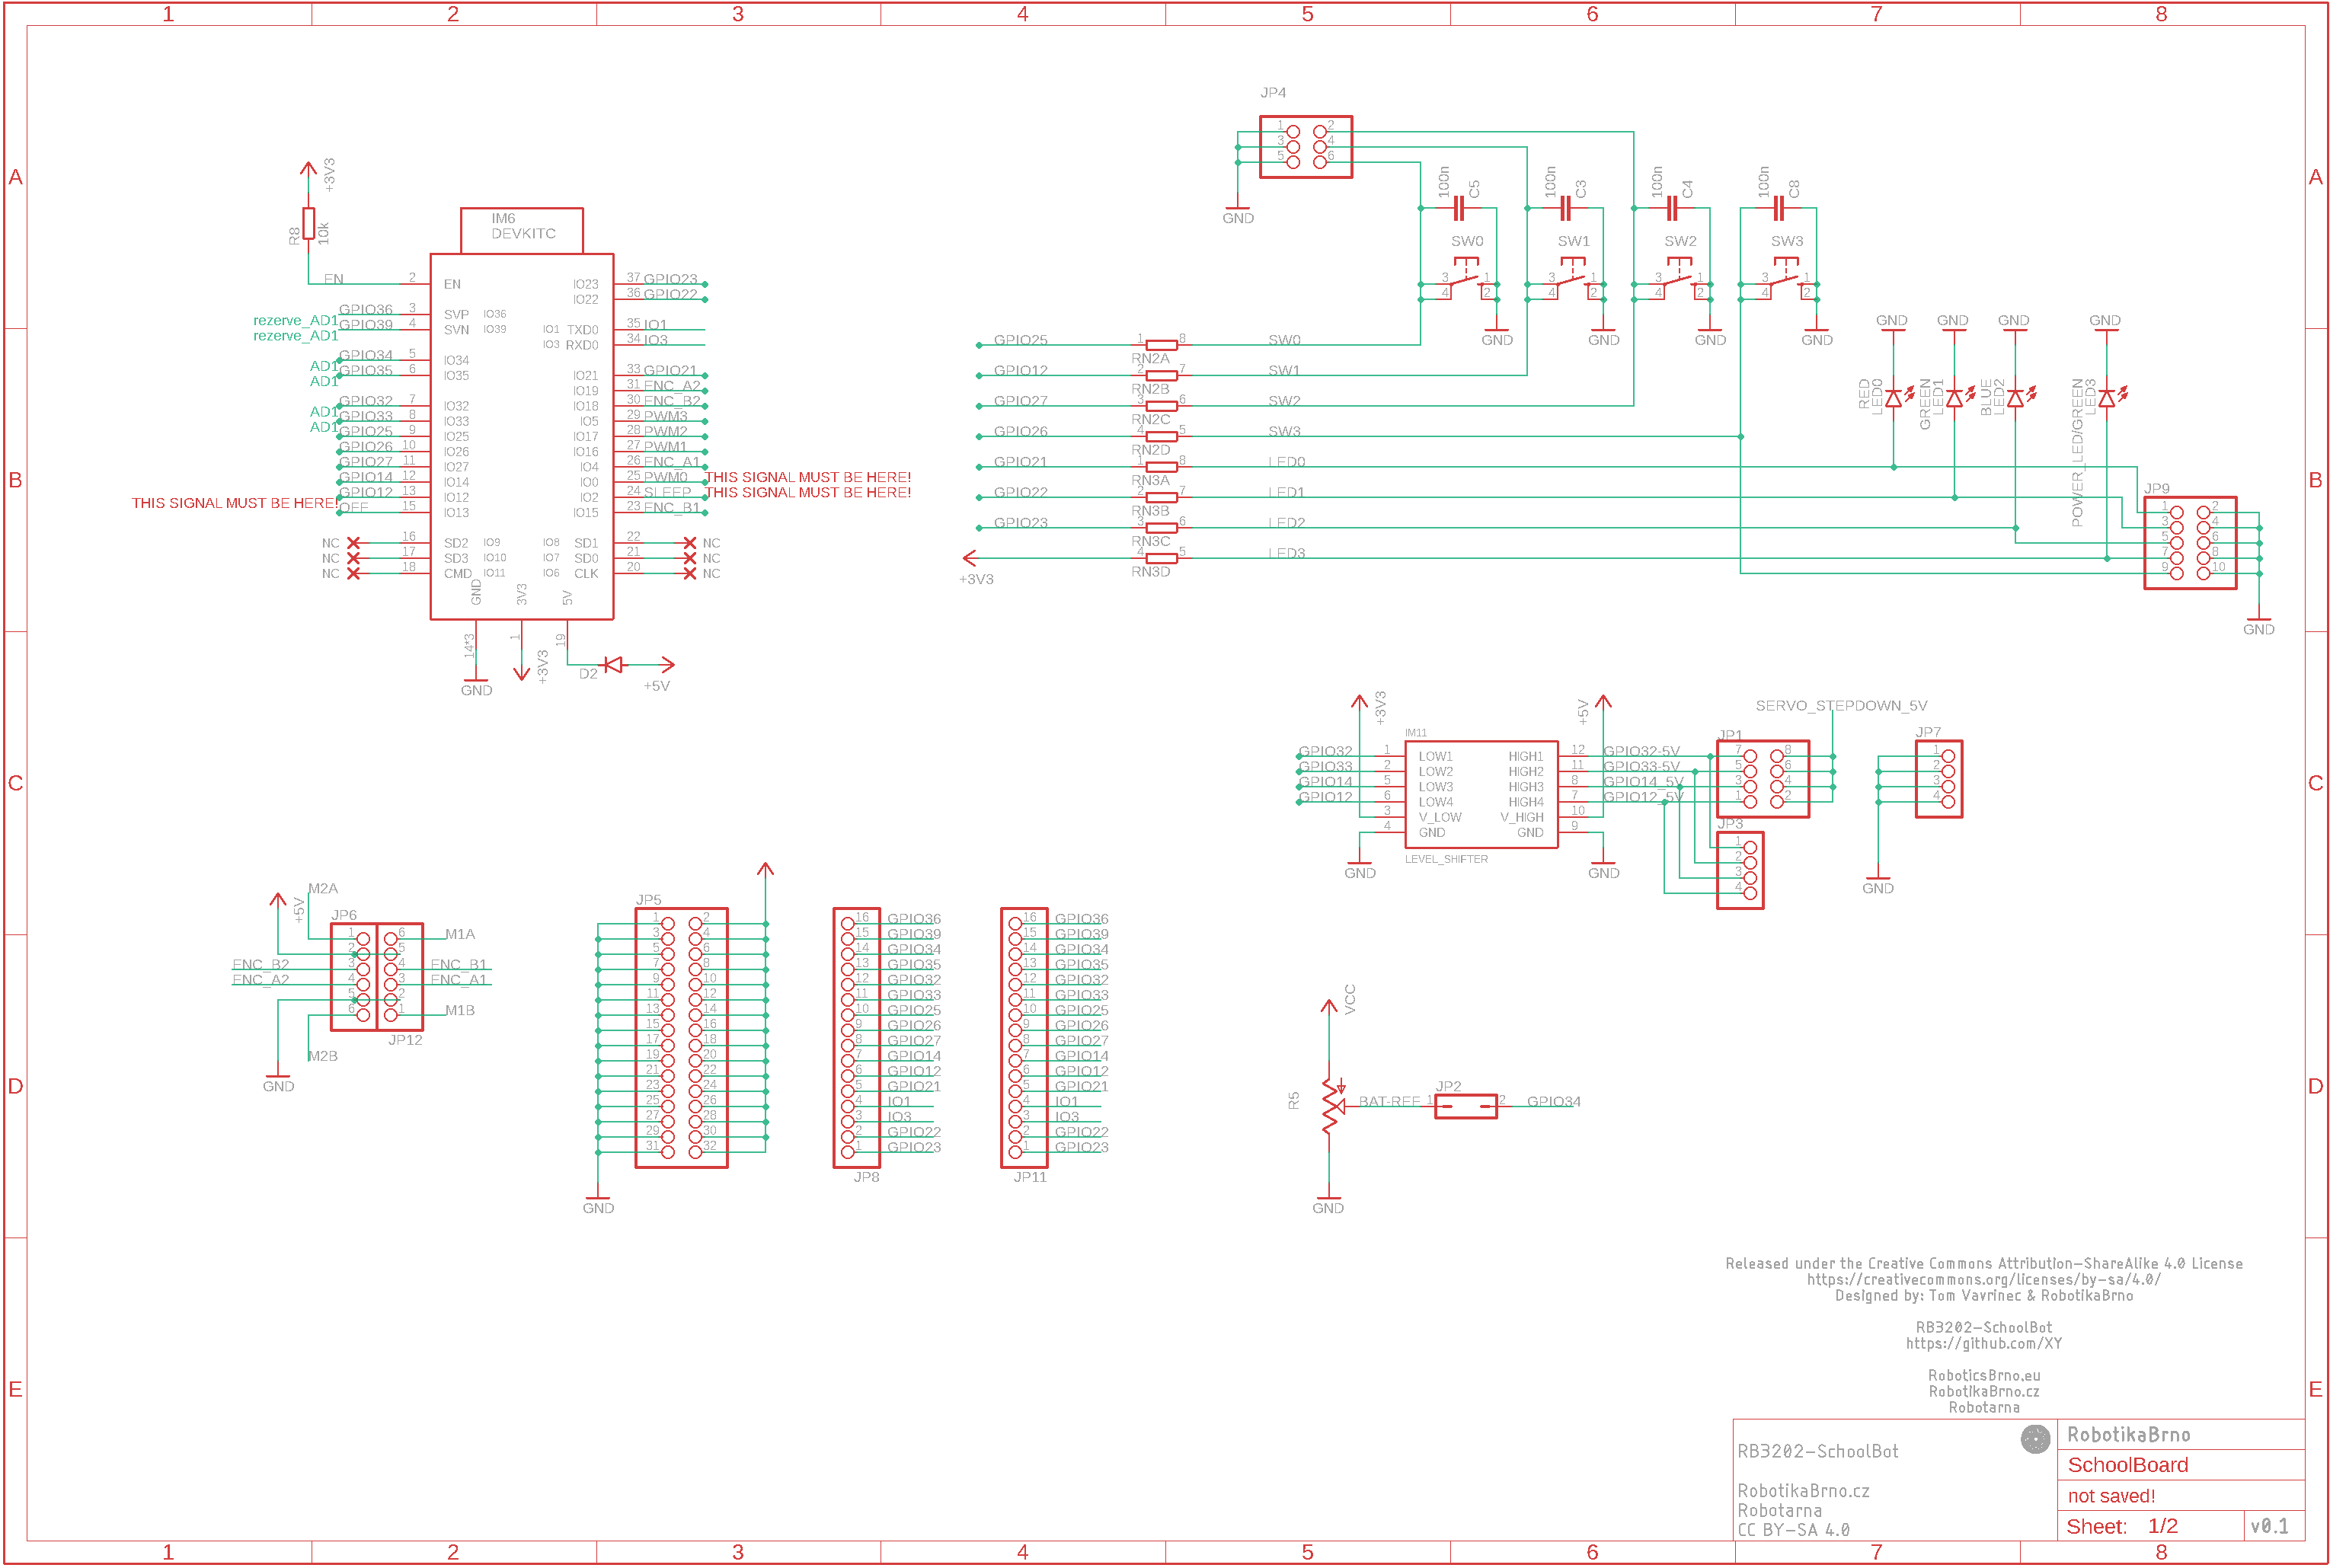
\includegraphics[width=\textwidth]{img/logika.png}
		\caption{schema logické části desky}
	\end{figure}
	
	\newpage
	
	\subsection*{DEVKIT C:}
	procesor ESP32 je v tomto případě osazený na devkitu C. Je to malá deska, která se stará o potřeby procesoru a dá se koupit jako celek. Zajišťuje jednoduché programování přes USB, zajištuje stabilizované napětí 3,3V pro ESP32 a 3,3V větev na desce a stará se o výchozí hodnoty na pinech u kterých je to potřeba.
	Seznam důležitých pinů
	\begin{itemize}
	\item EN – reset pin, pokud je na něm logická 0, ESP32 se resetuje, v normálním stavu na něm má být logická 1, proto je zde pull-up rezistor, který zajištuje logickou 1.
	
	\item Piny s označením reserv AD1 jsou vyhrazené pro externí použití 
	a nejsou tedy na desce nijak zapojené, jsou to piny, na které je připojený 
	první AD převodník ESP32 (ADC1), ADC1 je plně k užití pro uživatele na rozdíl 
	od ADC2, který je využíván Wi-Fi. ADC2 je tedy uživateli k dispozici, jen pokud jej zrovna nevyžaduje Wi-Fi.
	
	\item Piny s označením AD1 jsou také piny ADC1, ale jsou interně připojené na některé periferie, která však nemusí být použité
	
	\item \item IO34 – použitelná na měření napětí na baterii přes jumper JP2 přímo na desce
	\item \item IO35 – pin řídící inteligentní serva
	\item \item IO33, 32 jsou připojené na převodník napěťových úrovní pro možnost komunikovat na 5V. Analogové měření je ovlivněno pull-up rezistory na převodníku napěťových úrovní. Při potřebě užití těchto pinů jako analogových vstupů tedy doporučuji odebrat tyto pull-up rezistory. 
	To znamená, že tyto piny budou potřebovat softwarové pull-upy při užití jako vstupní pin při 5V komunikace.
	\item Piny s rudým označením THIS SIGNAL MUST BE HERE, jsou lehce problematické, protože ovlivňují boot ESP. Musí na nich tedy při bootu být správná logická hodnota, jinak by ESP mohlo třeba bootovat z jiné paměti nebo by třeba USB nemohlo zapisovat do paměti pro program. Piny IO0 a IO2 nejsou vyvedeny a je o ně interně postaráno, pin IO12 je ale vyveden a uživatel si tedy musí dát pozor, aby na něm neměl při bootu logickou 1. Pokud zůstane nepřipojen, deska se o něj postará.
	
	\subsection*{D2}
	Dioda sloužící k zamezení napájení 5V větve z USB.
	Ochrana před přetížením napájení z USB.
	
	\subsection*{RN3A, B, C, D:}
	rezistorová síť, odpory k ledkám.
	
	\subsection*{RN2A, B, C, D:}
	rezistorová síť, ochranné odpory ke tlačítkům, aby 
	byl procesor chráněn při případné chybě 
	v programu.
	
	\subsection*{SW0, 1, 2, 3:}
	uživatelská tlačítka
	
	\subsection*{C3, 4, 5, 8:}
	kondenzátory pro vyhlazení signálu z tlačítka při stisknutí
	
	\subsection*{JP4, 9:}
	vyvedení tlačítek a ledek ven z desky pro možnost	
	vyvedení dál od desky, např. deska muže být v útrobách robota, ale tlačítka a ledky mohou být 
	pořád pohodlně dostupné, protože jsou vyvedené	
	někam na povrch stroje.
	
	\subsection*{LED0, 1, 2:}
	ledky pro možnost signalizace různých stavů programu
	
	\subsection*{Led3:}
	powerled, signalizace, zda je deska zapnutá nebo vypnutá
	
	\subsection*{JP6, 12:}
	konektor pro připojení motoru s encoderem
	\item Vnější piny – napájení motoru
	\item Piny vedle vnějších pinů – napájení encoderu
	\item Vnitřní piny – signály encoderu
	\item Konektor je primárně určen pro inkrementální magnetické encodery, s nimi i počítají programové knihovny
	
	\subsection*{JP5:}
	vyvod 3.3V napájení
	
	\subsection*{JP8, 11:}
	vyvedení některých pinů ESP, každý pin je vyveden alespoň dvakrát pro možnost připojení osciloskopu pro příjemnější hledání chyb programu.
	
	\subsection*{LEVEL SHIFTER:}
	Neboli převodník napěťových úrovní zajištuje možnost digitální komunikace s 5V periferií pro čtyři piny ESP. Konkrétně pro piny IO32, IO33, IO14, IO12.
	\item IO32 – jeden z pinů ADC1, podrobněji u DEVKIT C.
	\item IO33 – jeden z pinů ADC1, podrobněji u DEVKIT C.
	\item IO14 – jeden z pinů ADC2. ADC2 je využíván Wi-Fi. Jinak není použit.
	\item IO12 – je nutno odstranit pull-up (na součástce převodníku). IO12 volí paměť,
	ze které se bootuje a jestli do té správné jde nahrát program. Jinak není interně použit.
	\item Všechny čtyři piny jsou jinak vyvedeny i ve variantě 3.3V.
	\item Převodník napěťových úrovní převádí logickou 1 pomocí pull-upů, tím pádem periferie pomocí převodníku spojené musí mít vstup s vysokým odporem, protože pokud by piny těchto periferií neměly velký odpor, tak by výsledek po dělení děliče vzniklého z pull-upu a periferie, která signál měří, mohl být pod rozlišovací schopností dané periferie.
	
	\subsection*{JP1, 3, 7:}
	vývody zpětivoltovaných pinu a jejich napájení
	\item Napájení 5V nemusí být nutně 5V, tyto piny mají vlastní stabilizaci napájení (IM3), a tím pádem záleží na tom, jak je tato stabilizace nastavená. Deska je primárně navržená pro dva způsoby stabilizace: 
	step-Down a stabilizátor řady 7805
	\item \item Step-Down má výhodu většího proudu, a hlavně nastavitelného napětí na výstupu. Naopak nevýhoda je nutnost nastavit požadované napětí a konkrétně u mnou používaného exempláře poměrně velký rozkmit výstupního napětí při změně odběru proudu.
	\item \item 7805 má výhodu napěťové stability naopak nevýhodu maximálního možného odebíraného proudu který závisí na vstupním napětí. Co se regulace napětí týče, v mnou použitém zapojení se napětí regulovat nedá.
	
	\subsection*{R5:}
	Trimr sloužící jako dělič napětí baterie pro možnost měření jejího napětí. 
	\textbf{Před použitím nutno nastavit na vhodnou dělící hodnotu vzhledem k použitým bateriím!} Na výstupu z děliče nesmí být při plně nabité baterii víc než 3,6V. Pokud se při daném použití desky nemá měnit maximální napětí na baterii (počet článků baterie nebo jejich druh), doporučuji nastavit trimr jednou a následně jej zalepit, aby se například vibracemi nemohl rozladit.
	
	\subsection*{JP2:}
	jumper pro možnost odpojení měření baterie za účelem uvolnění analogového pinu IO34. Zároveň se dá použít na měření výstupu z děliče před jeho zapojením k ESP.
	
	\section*{Silová čás}
	
	\begin{figure}[h]
		\centering
		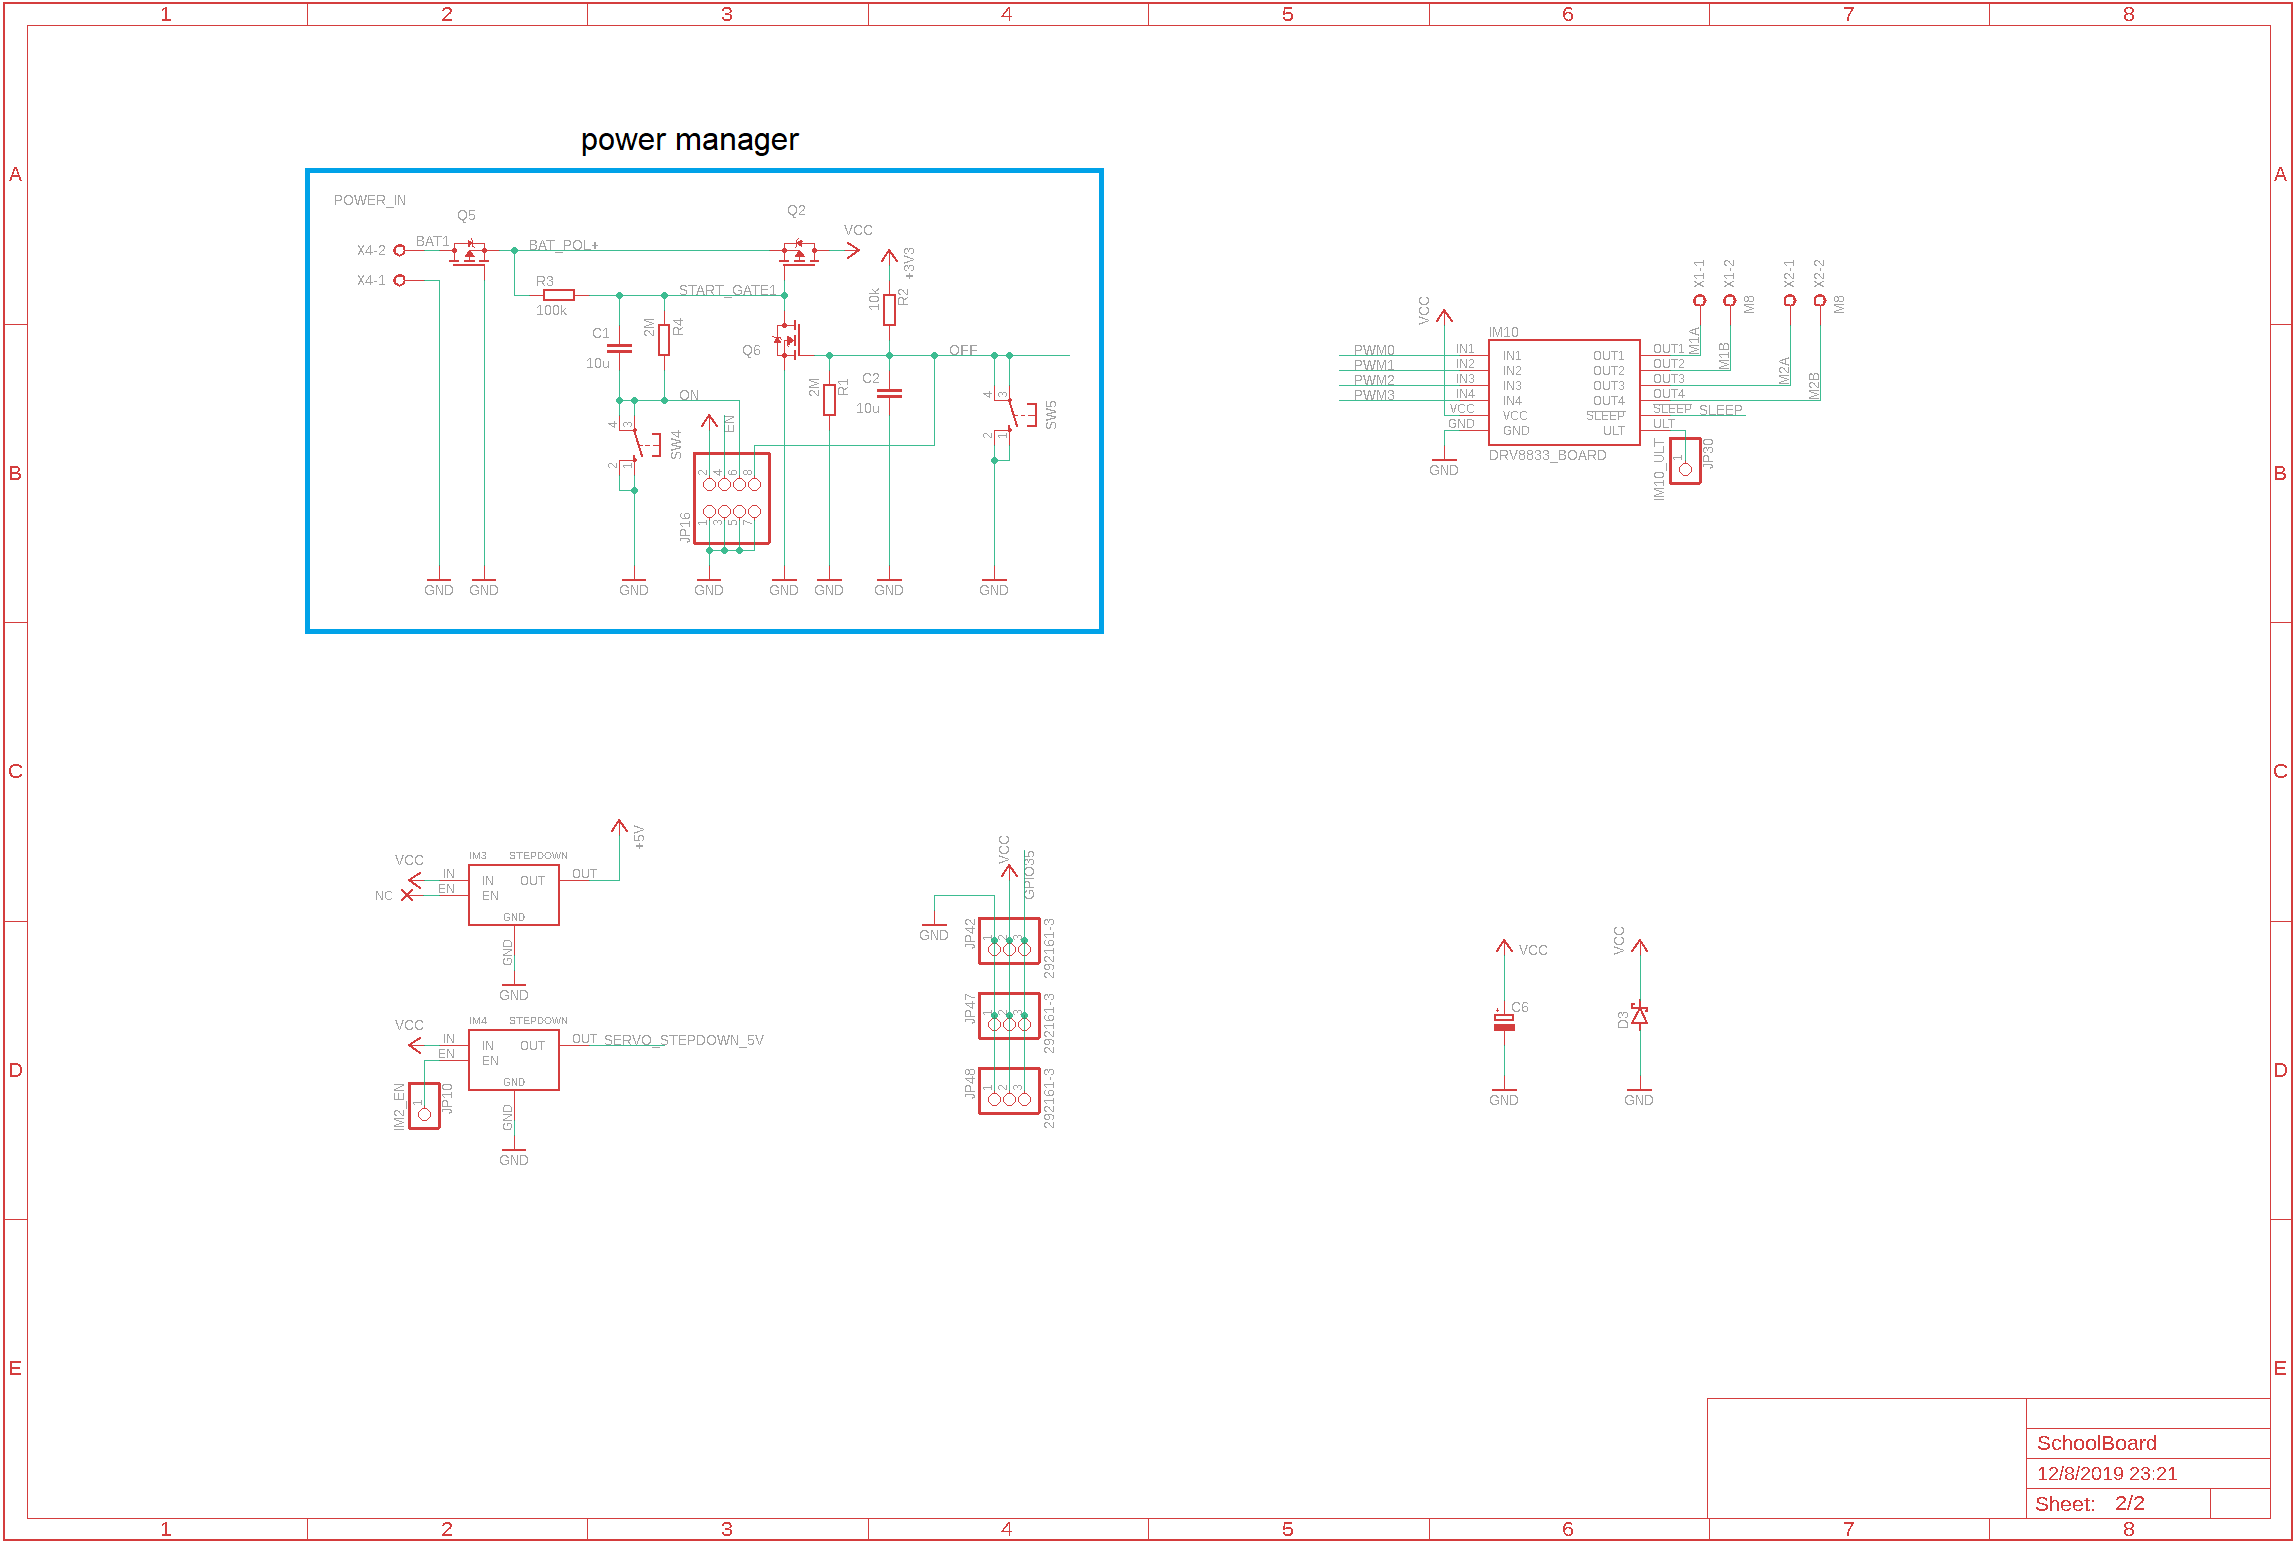
\includegraphics[width=\textwidth]{img/silovka.png}
		\caption{schéma výkonové části}
	\end{figure}

	\subsubsection*{Power manager:}
	
	\paragraph*{X4:}
	Svorkovnice pro připojení zdroje s napětím 7-11V. X4-1 je záporný pól a X4-2 je pól kladný.
	\paragraph*{Q5}
	MOSFET tranzistor typu P na ochranu proti přepólování
	
	Můžete si všimnout, že ochranná dioda uvnitř tranzistoru směřuje po směru proudu, a ne proti směru, což by bylo normální zapojení MOSFET tranzistoru.
	Tranzistor je zapojen takto právě z toho důvodu, že slouží jako ochrana proti náhodnému přepólování zdroje. Kdyby byl naopak, tak by sice při správné polaritě zdroje proud propustil a deska by byla napájena, ale v případě přepólování by proud propustil (skrz diodu) také, sice s ubytkem napětí na diodě, ale přes to by proud prošel a spálil by vše, co je citlivé na změnu polarity.
	\paragraph*{Q2}
	MOSFET tranzistor typu P, který umožnuje zapínání a vypínání desky
	\paragraph*{R3}
	Pull-up na bateriové napětí pro dráhu START~GATE1
	\paragraph*{Q6}
	MOSFET tranzistor typu N řídící tranzistor Q2
	\paragraph{R2}
	Pull-up na 3.3V pro dráhu OFF
	\item V zapnutém stavu drží na dráze OFF 3.3V
	(ne úplně čisté napětí ze stabilizátoru na ESP kvůli pull-downu R1) a tím otvírá tranzistor Q6, který zas drží otevřený tranzistor Q2.
	
	\paragraph*{R1}
	Pull-down pro dráhu OFF
	\item Tento rezistor je zde pro plné definování dráhy OFF,
	a to i ve stavu, kdy ESP není zapojeno, tím pádem by dráha nebyla jasně určena.
	
	\paragraph*{SW5}
	Tlačítko, které připíná dráhu OFF k zemi, a tím zavírá tranzistor Q6, čímž vypíná desku.
	
	\paragraph*{SW1}
	Tlačítko připínající dráhu ON k zemi, čímž skrz kondenzátor C1 a tranzistor Q2 zapne stabilizátor na DEVKIT-C, který pomocí rezistoru R2 otevře tranzistor Q6, který otevře Q2. 
	
	\paragraph*{C1}
	Kondenzátor, který se nabije při stisku tlačítka SW4, čímž na dobu nabíjení přivede na dráhu START~GATE zem a tím krátkodobě otevře tranzistor Q2. Přes Q2 projde proud, který pomocí stabilizátoru na DEVKIT-C vytvoří 3,3V, skrz pul-up R2 otevře tranzistor Q6 a ten trvale otevře tranzistor G2.Deska je v tu chvíli zapnutá.
	
	\paragraph*{R4}
	Rezistor pro vybíjení kondenzátoru C1
	
	\paragraph*{JP6}
	Konektor, pro možnost vyvedení vypínaní, zapínání, resetu 
	a kontrolní powerledky na externí ovládání.
	
	\paragraph*{Obvod jako celek}
	Po připojení zdroje s napětím mezi 7 až 11V se při špatné polaritě napětí nedostane skrz tranzistor Q5. Deska sice nejede, protože nemá napájení, ale je chráněna před zničením opačnou polaritou. Při správném připojení zdroje, napětí projde skrz Q5 a tím pádem je na drahách BAT~POL+, START~GATE1 a ON napětí zdroje, na VCC se napětí nedostane, protože tranzistor Q2 je zavřen. Při stisku tlačítka SW4 se na dráhu ON dostane zem, tím pádem se kondenzátor C1 nabije a při nabíjení krátkodobě otevře tranzistor Q2. V době, kdy je tranzistor Q2 otevřen, skrz kondenzátor C1, se pomocí stabilizátoru osazeném na DEVKITu-C vytvoří napětí 3.3V. Skrz pul-up R2 se dostanou 3.3V na dráhu OFF a tím pádem na Gate tranzistoru Q6, který se v tu chvíli otevře a trvale přivede zem na dráhu START~GATE1. V tuto chvíle je tranzistor Q2 trvale otevřen, až do doby, kdy se na dráhu OFF nepřivede zem, v tu chvíli se zavře tranzistor Q6 protože má na Gate stejné napětí jako na Source (oba piny je připojené k zem). Pokud je Q6 zavřený zbývá jen možnost připojení země odjinud, pokud uvažujeme tento obvod bez poškození nebo jakéhokoli doplnění. Skrz rezistor R3 je dráha START~GATE1 připojena na zdrojové napětí, tím pádem je tato dráha tahána ke kladnému pólu a na k pólu zápornému, což by bylo potřeba pro otevření tranzistoru Q2, tímto způsobem se tedy Q2 určitě neotevře.
	START~GATE1 je dále připojen na rezistor R4 a kondenzátor C1 které jsou dále připojeny na přes tlačítko SW4 k zemi. Pokut je tedy tlačítko SW4 spojeno se zemí je zem i na dráze ON, v tuto chvíli je sice na dráhu 
	STERT~GATE1 skrz R4 připojena zem, ale vzhledem
	k tomu že R4 má desetkrát větší odpor než R3, který spojuje dráhu START~GATE s bateriovým napětím, na Gate tranzistoru Q2 pořád nebude dostatečně malé napětí, aby se Q2 otevřel. C1 propustí proud jen po dobu jeho nabíjeni a tím pádem se skrz nej nedá deska udržet trvale otevřená, dá se jím jen zapnout. To znamená že pokud procesor napíše na pin připojený na dráhu OFF, IO13, logickou nulu, deska se vypne, bez ohledu na to, jaké tlačítko člověk drží. Vypínání ne nutně platí pro 3.3V větev která je napájena jak z baterie tak z micro-USB na DEVKITu-C, takže pokud je procesor připojen k počítači pravděpodobně za účelem programování procesor a vše co je napájené z 3.3V je nadále funkční. Pokud USB není zapojeno, pak se při stisku SW5 nebo zápisu logické 0
	na pin IO13 deska jednoduše kompletně vypne.
	
	\subsubsection*{IM10}
	Motorový driver, DRV8833, na řízení dvou stejnosměrných motorů v napěťovém rozsahu 2,7 až 11V a maximálním proudem 1,5A. 
	Driver je také schopný místo dvou stejnosměrných motorů řídit jeden krokový motor.
	DRV8833 má pět vstupních řídících pinů: čtyři IN piny (dva pro každý motor) a sleep pin.  Podle IN pinů se řídí výstup - viz tabulka.
	Sleep pin uvádí driver do sleep módu pokud je připojen k zemi. Sleep mód slouží uživateli k úspoře energie v době, kdy nepotřebuje ovládat motory (po dobu aktivního sleep modu zůstanou motory pochopitelně vypnuté).
	
	\begin{table}[h]
		\centering
		\begin{tabular}{|l|l|l|l|l|}
			\hline
			xIN1 & xIN2 & xOUT1 & xOUT2 & FUNCTION \\ \hline
			0 & 0 & Z & Z & Coast/fast decay \\ 
			0 & 1 & L & H & Reverse \\ 
			1 & 0 & H & L & Forward \\ 
			1 & 1 & L & L & Brake/slow decay \\ 
			\hline
		\end{tabular}
		\caption{}
	\end{table}
	\newpage
	\subsubsection*{X1, X2}
	Svorkovnice na silové vývody k motorům.
	
	\subsubsection*{IM3}
	Step-down/stabilizátor pro 5V větev
	\item 5V napájí ESP, tím pádem i celou 3.3V větev skrz DEVKIT C
	\item Napětí, které je, zde je zároveň i napětí, na kterém komunikují 5V piny, proto doporučuji sem dát stabilizátor 7805, u kterého nemusíte hlídat napětí.
	
	\subsubsection*{IM4}
	Step-down/stabilizátor pro napájení 5V pinů na 5V piništi.
	
	\subsubsection*{JP42, 47, 48}
	Konektory pro připojení inteligentních serv.
	\item Navrženo pro serva LX-16A a LX-15D
	
	\subsubsection*{C6}
	Velký elektrolytický kondenzátor jako zásobárna proudu při náhlé změně odběru.
		
	\subsubsection*{D3}
	Zpětná dioda pro případ napěťové špičky, která by krátkodobě převrátila polaritu. V takovém případě se dioda otevře a proud propustí skrz sebe místo, aby protekl jinudy a přitom něco zničil.
	
	\end{itemize}


	\part*{Vysvětlení některých pojmu pro začátečníky}
	
	\chapter*{Důležité elektronické součástky}
	\section*{Dioda}
	Dioda je polovodičová součástka, která vede proud jenom jedním směrem. Dioda obsahuje PN přechod, který zajištuje její schopnost vest proud jen jednosměrně. Pokud nás zajímá, jak je dioda schopna vést proud můžeme se pro konkrétní diodu podívat na její voltampérovou charakteristiku. Pro všechny diody však budou platit několik bodu (s ohledem na napětí) kde se bude křivka zásadně měnit. Je to prahové napětí, a napětí průrazu. Prahové napětí je napětí, při kterém se dioda otevře, žádná dioda totiž není ideální a ani kladné napětí jí neprojde, pokud není dostatečně velké. Pro obyčejné diody většinou bývá menší než jeden volt (někdy se uvádí 0.6V, ale rozhodně to neplatí vždy). Ale například u LED diod je téměř vždy vyšší, konkrétně třeba u modře svítících bývá i přes dva a půl voltu.
	Diody mají několik různých typů. Každý typ se hodí na jinou aplikaci. Například Zenerova dioda má výhodu vtom, že po průrazu není zničena a pokud napětí opět klesne, její funkce se obnoví. Její nevýhoda je však velká kapacita. Z podobných důvodů je každá dioda vhodná pro jinou aplikaci.
	Zenerova dioda – Po průrazu není zničená, takže se dá využít třeba jako napěťová ochrana. Její nevýhodou většinou bývá velké kapacita.
	Schottkyho dioda – Dokáže se velice rychle otevřít i zavřít (velmi rychle reaguje na změnu polarity) má však velký zpětný proud. Schottkyho dioda totiž není tak úplně dioda, nemá totiž žádní PN přechod.
	Fotodioda – Dioda, která má velký PN přechod a má průsvitné pouzdro. PN přechod totiž nereaguje jen na elektřinu, ale je citlivý i na světlo (kromě fotodiod jsou proto diody v neprůsvitném pouzdře). Díky tomu se fotodioda dá využít jako detektor světla a aby se tento jev dal využít ještě lépe, 
	je přechod oproti jiným diodám zvětšen.
	\section*{MOSFET}
	Zkratka vyjadřuje:
	M (Metal) – elektroda G je tvořena kovem (hliníkem)
	O (Oxide) – elektroda G je odizolována vrstvičkou oxidu křemičitého
	S (Semiconductor) – oxid je vytvořen na polovodičové destičce
	FET (Field effect transistor) – výsledkem je tranzistor řízený napětím UGS
	MOSFET (Metal Oxide Semiconductor Field Effect Transistor)
	MOSFET je druh tranzistorů, který je řízen elektrickým polem. Tranzistor je speciální tím, že má elektrodu G (Gate) od zbytku tranzistoru odizolovanou tenkou vrstvou oxidu křemičitého. To má za následek především to, že elektrodou G neteče teoreticky žádný proud. Na základě znalostí o bipolárních tranzistorech by si člověk mohl asi říct, že takovýto tranzistor přece nebude fungovat, protože přece proud bází určuje proud emitorem, takže pokud bází nepoteče nic tak emitorem taky ne. Ale MOSFETy jsou řízeny napětím. Napětím mezi G (Gate, vlastně báze akorát u MOSFETu se nazývá jinak) a S (Source, vlastně emitor), které se pak označuje jako UGS.
	Elektroda G totiž vytváří elektrické pole, které vytváří vodivý kanál uvnitř tranzistoru. Vzniklé pole totiž odpuzuje/přitahuje kladné díry/záporné elektrony, čímž vytváří v jinak nevodivé oblasti nasycení na PN přechodu vodivou oblast.
	Běžný MOSFET je MOSFET s indukovaným kanálem, to znamená že vodivá oblast (kanál) existuje jen pokud existuje dostatečně velké napětí UGS správné polarity (pro N MOSFET kladné a pro P MOSFET záporné).  Existují ale i MOSFETy s technologicky vytvořeným kanálem. Takové tranzistory mají vytvořený mezi elektrodami S a D vodivý kanál tvořený prostředím se stejným typem vodivosti. To pak umožnuje tranzistoru pracovat ve dvou režimech, režimu obohacení a režimu ochuzení. V režimu obohacení se vodivý kanál, díky elektrostatickému náboji tvořenému pomocí elektrody G, dále rozšiřuje a umožnuje tak protékat většímu proudu. V režimu ochuzení se však kanál naopak zužuje a omezuje tak průtok proudu.
	Na všech obrázcích jsou MOSFET typu P, pokud si chcete představit MOSFET typ N, musíte si u všech obrázků představit opačné napětí UGS, aby platily pro typ N.
	
	
	\chapter*{Důležité pojmy}
	
	\section*{Pin}
	Pin je vývod elektrické součástky.
	Pull-up
	Pull-up je rezistor, který připojuje logickou dráhu k napájení. Pokud měříme napětí na takovéto dráze (když není nikam jinam připojena) pomocí měřidla s vysokým odporem (což bude každý pin nastavený jako vstupní) naměříme prakticky napájecí napětí. 
	Toto se využívá například při čtení tlačítka, které je pak připojeno dvěma vodiči, z nichž jeden je připojen na zem a druhý je připojen zaprvé na pin procesoru a zadruhé přes pull-up k napájení. 
	Pokud pak čteme tento pin, přečteme logickou jedničku, když tlačítko nebude stlačené a logickou nulu, když stlačené bude.
	
	\section*{Pull-down}
	Pull-down je stejně jako pull-up rezistor, který určuje napětí na logické dráze, ale na rozdíl od
	pull-upu připojuje dráhu k zemi.
	Co je analogový a digitální signál
	Digitální signál reprezentuje logické hodnoty, 0 nebo 1. Má tedy dva možné stavy. Analogový signál může naopak nabývat teoreticky nekonečně mnoha hodnot, protože je vyjádřen napětím, které může nabývat jakékoliv hodnoty v daném rozsahu. V praxi se většinou analogový signál převádí pomocí AD převodníku na digitální podobu, aby s takovýmto vstupem byl procesor schopen pracovat.
	Technický list desky SchoolBoard
	
	\section*{Napěťový dělič}
	Odvození vzájemného vztahu mezi napětím a odpory rezistoru.
	\begin{listedequation}[h]
		$$I=U{1}/R{1}$$
		\caption{stejně tak}
		$$I=U{2}/R{2}$$ 
		\caption{z toho plyne}
		$$U{1}/U{2} =R{1}/R{2}$$
		\label{eq:hrnekeq}
	\end{listedequation}
	 		
	Napětí na rezistorech se tedy dělí v poměru jejich odporu. V praxi v obvodu nebudou jen dva rezistory, ale aby dělič k něčemu byl, je na uzlu mezi rezistory měřeno referenční napětí. Pro výpočet se dá měřidlo nahradit dalším rezistorem zapojeným paralelně k R2. Tento další rezistor můžeme ve většině případů zanedbat, protože měřidla napětí budou většinou mít velký vnitřní odpor a tím pádem skrz ně nepoteče velký proud. Ale kdybychom měřidlo uvažovali, tak by platilo:
	
	\begin{listedequation}[h]
		$$U{1}/U{2} =R{1}/R{2,3}$$
		\caption{kde R{2,3}}
		$$1/R{2,3} =1/R{2} +1/R{3}$$ 
		\caption{Kde R3 je odpor měřidla (pravděpodobně bude v řádu megaohmu)}
		\label{eq:hrnekeq}
	\end{listedequation}
	
	\section*{Enkodér}
	Enkodér je snímač polohy. Většinou se používá pro určení natočení motoru. Pomocí něj se dá počítat například úhlová rychlost motoru, nebo ve spojitosti s dalšími senzory třeba okamžitý výkon nebo kroutící moment. 
	Enkodéry se dají rozdělit do dvou hlavních skupin, inkrementální a absolutní. 
	Inkrementální enkodéry dávají informaci o velikosti posuvu a jeho směru.
	Absolutní enkodéry udávají jeho reálnou pozici (jsou většinou daleko složitější než inkrementální).
	
	\subsection*{Inkrementální enkodéry}
	Inkrementální enkodéry jsou, stejně jako ostatní druhy enkodérů, zdrojem informací o poloze, většinou motoru. Rozlišení je definováno počtem impulzů na otáčku, které enkodér při každé otáčce vytvoří. Aktuální pozice pak vlastně známá není, jen pokud se zjistí jiným snímačem. Enkodér vlastně říká, kterým směrem a o jaký úhel se rotor otočil. Takový enkodér má alespoň dvě sondy, na signálu posunuté o 90 stupňu (viz obrázek), které snímají pohyb rotoru. Snímání je pak zajištěno buď opticky, magneticky nebo u malých rychlostí i mechanicky. Mají velmi jednoduchou logiku vyhodnocování. Magnetická verze inkrementálního enkodéru má na rotoru, nebo jiném pohyblivém zařízení, umístěn magnet, jehož magnetické pole se snímá pomocí Hallových sond. Tento magnet pak určuje rozlišení enkodéru. Pokud má enkodér jen jeden magnet, má pak jen dvě hrany na otáčku sestupnou a vzestupnou, které jsou v případě ideálního magnetu stejně vzdálené. Stejná vzdálenost hrany na otáčku značí, že signál sondou vygenerovaný, bude o polovinu otáčky hight a polovinu low. Pokud tedy chceme větší rozlišení, musíme buď otáčky magnetu nějak z převodovat, což má nevýhodu vůlí, kterým je u převodovek těžké se vyhnout. Nebo musí být “magnet“ složen z většího počtu magnetů, aby měl výsledek větší počet pólů na otáčku.
	
	Optické inkrementální enkodéry jsou oproti magnetickým daleko běžnější. Používají se například ve většině počítačových myší. Nepotřebují magnety, ale jen nějakou clonu nebo odraznou plochu. Clona nebo odrazka pak umožní ve správném natočení, dostat se světlu do jeho snímače, většinou phototransistoru.
	Disk na obrázku může být buď neprůsvitný a mýt v sobě otvory, nebo může být transparentní a mít na sobě jen nakreslené neprůsvitné nebo přímo odrazné plošky. Při odrazné možnosti je pak možné snímat natočení ze stejné strany, na které je umístěn zdroj světla. Podobný způsob může využívat například různé odraznosti barev, například na disku mohou být natištěny různě barevné plochy, které budou různě pohlcovat světlo a tedy se do snímače dostane různé množství světla. 
	Mechanické enkodéry mechanicky připínají výstupy k dané dráze, stejně jako u tlačítek je touto dráhou většinou zem. Proč zrovna zem? Protože logická nula je ve většině případů právě zem a pokud musíme jednu ze stavů definovat, je lepší určit ten, který nám umožní větší flexibilitu. Signál pak připojíme přes pull-up k logickému napájení, který si už ale můžeme téměř libovolně zvolit. 
	Co se vzhledu rotačního disku týče, přirovnal bych je k enkodéru optickému. Vlastně se dá říci, že místo světla se zde pohybuje elektřina (i když to není tak úplně přesné).
	
	\subsection*{Absolutní enkodéry}
	Absolutní enkodéry udávají na rozdíl od inkrementálních reálnou polohu rotoru. Dávají nám tedy informaci o aktuálním natočení, nikoli o posunu jako ty inkrementální. Rozlišení se pak tedy neodvíjí od množství hran na otáčku, ale od schopnosti rozlišit úhel natočení (rozvedeno níže). Stejně jako enkodéry inkrementální mohou být i absolutní magnetické i optické a mohou být i mechanické (ty se téměř nepoužívají). Za mechanické absolutní enkodéry by se dali v jistém smyslu považovat potenciometry. Ty se ale málokdy dělají tak, aby s nimi bylo možné točit dokola při zachování informace o poloze. Magnetické absolutní enkodéry využívají opět Hallova jevu, ale na rozdíl od inkrementálního enkodéru nepřevádí výstupní signál na digitální, ale ženou jej na AD převodník. Díky tomu mají oproti inkrementálním enkodérům daleko přesnější informaci, ale zase obtížněji zpracovatelnou. Magnetické pole snímaného magnetu totiž sice může být velmi stálé, ale je téměř nemožné jej dokonale odstínit. Signál tak bude obsahovat všelijaké rušení (například běžící motor), které je třeba nějak odfiltrovat, jinak bude podstatně snižovat přesnost enkodéru. Jeho rozlišení pak vyplývá z přesnosti AD převodníku a ze schopnosti odstínit nebo vyfiltrovat měřený signál. Optické absolutní enkodéry mají oproti inkrementálnímu daleko složitější disk. Přesnost takovéhoto enkodéru pak určuje množství bitů, na kterých poskytuje informaci o natočení disku. Dalo by se říci, že pokud je enkodér řekněme osmibitový (viz obrázek) skládá se z osmi různých inkrementálních enkodérů s různou přesností, které na sebe jedinečným způsobem navazují.	Když se podíváte na obrázek A, můžete si všimnout, že od středu disku narůstá počet hran na otáčku. Dále si můžete všimnout, že kombinace pruhu je pro každý úhel jedinečná - v případě tohoto obrázku s přesností na 360 stupňu lomeno 256 (256 protože enkodér umožnuje rozlišení na osm bitech). Právě díky jedinečnosti informace pro každý úhel je enkodér absolutní, protože když při libovolném natočení, přečteme výstup, dokážeme určit, jak je zrovna enkodér natočen.
	
	\section*{PWM}
	Pulse Width Modulation (Pulzní šířková modulace) je obdélníkový signál s proměnlivým poměrem vysokého a nízkého stavu. Tento poměr se pak nazývá procento PWM. Pokud je signál stále v poloze nízké, je nula procentní, a pokud je naopak stále vysoko, je sto procentní.
	PWM se využívá například při řízení svítivosti ledek. Ledka vlastně velmi rychle bliká, ale lidskému oku se zdá, že svítí méně intenzivně. 
	Větší využití má PWM v silové elektronice konkrétně při řízení stejnosměrných motoru. Pomocí PWM se totiž dá jednoduše řídit výkon motoru, motor je vlastně stejně jako ledka střevě zapnutý a vypnutý. To se však děje tak rychle, že se motor nestihne zastavit ani dosáhnout plného výkonu.
	
	\section*{Převodník napěťových úrovní}
	Převodník napěťových úrovní slouží k možnosti převádět digitální signál mezi dvěma různými systémy, které normálně komunikují na odlišném napětí.
	
	\subsection*{Funkce}
	
	\paragraph*{Komunikace z nízkého na vyšší napětí}
	Pokud napíše, řekněme procesor (provozován na napětí LV), na stranu napětí LV (low voltage) logickou nulu, tedy ji připojí na zem. Bude napětí GS rovno LV (napájecí napětí procesoru), protože G Q1 je připojena
	k LV a na S je v tu chvíli napsaná nula (zem). Tím pádem je Q1 otevřen a zem projde skrz Q1. Pokud však procesor napíše místo nuly jedničku, bude napětí GS 0V. V tu chvíli je Q1 zavřen a dráha s vyšším napětím je tažena pull-up rezistorem R9 k HV (hight voltage) => na dráze je logická jedna.
	
	\paragraph*{Komunikace z vyššího napětí na nižší}
	Pokud napíše, řekněme periferie napájena napětím HV, nulu. Signál projde skrz diodu uvnitř Q1, tím sníží napětí na S Q1 a plně Q1 otevře. Protože napětí GS je v tu chilli rovno LV. Pokud napíše periferie logickou jedna, napětí neprojde skrz Q1 a dráha LV-S je tažena pull-up rezistorem R8 k napětí LV.
	
	

\end{document}



odkladiště 




rady jak psát atd.


\chapter{Jak psát}
Abychom mohli napsat odborný text jasně a srozumitelně, musíme splnit několik základních předpokladů\cite{vut-zkousky}:
\begin{itemize}
	\item musíme mít co říci,
	\item musíme vědět, komu to chceme říci,
	\item musíme si dokonale promyslet obsah,
	\item musíme psát strukturovaně.
\end{itemize}

\section{Musíme mít co říci}
Nejdůležitějším předpokladem dobrého odborného textu je myšlenka.
Je-li myšlenka dost závažná, tak přetrvá, i když je neobratně a zmateně podaná.
Chceme-li však myšlenku podat co nejvýstižněji a ušetřit tak čtenáři čas, musíme dodržet určité zásady, o~kterých pojednáme dále.

\section{Musíme vědět, komu to chceme říci}
Dalším důležitým předpokladem dobrého psaní je psát pro někoho.
Píšeme-li si poznámky sami pro sebe, píšeme je jinak než výzkumnou zprávu, článek, diplomovou práci, knihu nebo dopis.
Podle předpokládaného čtenáře se rozhodneme pro způsob psaní, rozsah informace a míru detailů.

\section{Musíme si dokonale promyslet obsah}
Jakmile víme, co chceme říci a komu, musíme si rozvrhnout látku.
Ideální je takové rozvržení, které tvoří logicky přesný a psychologicky stravitelný celek, ve kterém je pro všechno místo a jehož jednotlivé části do sebe přesně zapadají.
Jsou jasné všechny souvislosti a je zřejmé, co kam patří.

Abychom tohoto cíle dosáhli, musíme pečlivě organizovat látku.
Rozhodneme, co budou hlavní kapitoly, co podkapitoly a jaké jsou mezi nimi vztahy.
Diagramem takové organizace je graf, který je velmi podobný stromu, ale ne řetězci.
Při organizaci látky je stejně důležitá otázka, co do osnovy zahrnout, jako otázka, co z~ní vypustit.
Příliš mnoho podrobností může čtenáře právě tak odradit jako žádné detaily.

\section{Musíme začít psát strukturovaně}
Máme-li tedy myšlenku, představu o~budoucím čtenáři, cíl a osnovu textu, můžeme začít psát.
Při psaní prvního konceptu se snažíme zaznamenat všechny své myšlenky a názory vztahující se k~jednotlivým kapitolám a podkapitolám.
Každou myšlenku musíme vysvětlit, popsat a prokázat.
Hlavní myšlenku má vždy vyjadřovat hlavní věta a nikoliv věta vedlejší.


\chapter{Několik formálních pravidel}
Naším cílem je vytvořit jasný a srozumitelný text.
Vyjadřujeme se proto přesně, píšeme dobrou češtinou (nebo zpravidla angličtinou) a dobrým slohem podle obecně přijatých zvyklostí.
Text má upravit čtenáři cestu k~rychlému pochopení problému, předvídat jeho obtíže a předcházet jim.
Dobrý sloh předpokládá \B{bezvadnou gramatiku, správnou interpunkci a vhodnou volbu slov.} Snažíme se, aby náš text nepůsobil příliš jednotvárně používáním malého výběru slov a tím, že některá zvlášť oblíbená slova používáme příliš často.
Pokud používáme cizích slov, je samozřejmým předpokladem, že známe jejich přesný význam.
Ale i českých slov musíme používat ve správném smyslu.
Např.
platí jistá pravidla při používání slova zřejmě.
Je zřejmé opravdu zřejmé? A~přesvědčili jsme se, zda to, co je zřejmé opravdu platí? Pozor bychom si měli dát i na příliš časté používání zvratného se.
Například obratu dokázalo se, že… zásadně nepoužíváme.
Není špatné používat autorského my, tím předpokládáme, že něco řešíme, nebo například zobecňujeme spolu se čtenářem.
V~kvalifikačních pracích použijeme autorského já (například když vymezujeme podíl vlastní práce vůči převzatému textu), ale v~běžném textu se nadměrné používání první osoby jednotného čísla nedoporučuje.

Za pečlivý výběr stojí i \B{symbolika}, kterou používáme ke značení.
Máme tím na mysli volbu zkratek a symbolů používaných například pro vyjádření typů součástek, pro označení hlavních činností programu, pro pojmenování ovládacích kláves na klávesnici, pro pojmenování proměnných v~matematických formulích a podobně.
Výstižné a důsledné značení může čtenáři při četbě textu velmi pomoci.
Je vhodné uvést seznam značení na začátku textu.
Nejen ve značení, ale i v~odkazech a v~celkové tiskové úpravě je důležitá důslednost.

S~tím souvisí i pojem z~typografie nazývaný \B{vyznačování}.
Zde máme na mysli způsob sazby textu pro jeho zvýraznění.
Pro zvolené značení by měl být zvolen i způsob vyznačování v~textu.
Tak například klávesy mohou být umístěny do obdélníčku, identifikátory ze zdrojového textu mohou být vypisovány písmem typu psací stroj.

Uvádíme-li některá fakta, neskrýváme jejich původ a náš vztah k~nim.
Když něco tvrdíme, vždycky výslovně uvedeme, co z~toho bylo dokázáno, co teprve bude dokázáno v~našem textu a co přebíráme z~literatury s~uvedením odkazu na příslušný zdroj.
V~tomto směru nenecháváme čtenáře \B{nikdy na pochybách}, zda jde o~myšlenku naši nebo převzatou z~literatury.

Nikdy neplýtváme čtenářovým časem výkladem triviálních a nepodstatných informací.
Neuvádíme rovněž několikrát totéž jen jinými slovy.
Při pozdějších úpravách textu se nám může některá dříve napsaná pasáž jevit jako zbytečně podrobná, nebo dokonce zcela zbytečná.
Vypuštění takové pasáže nebo alespoň její zestručnění přispěje k~lepší čitelnosti práce! Tento krok ale vyžaduje odvahu zahodit čas, který jsme jejímu vytvoření věnovali.

\chapter{Nikdy to nebude naprosto dokonalé}
Když jsme už napsali vše, o~čem jsme přemýšleli, uděláme si den nebo dva dny volna a pak si přečteme sami rukopis znovu.
Uděláme ještě poslední úpravy a skončíme.
Jsme si vědomi toho, že \B{vždy zůstane něco nedokončeno}, vždy existuje lepší způsob, jak něco vysvětlit, ale každá etapa úprav musí být konečná.

\chapter{Typografické a jazykové zásady}
Při tisku odborného textu typu technická zpráva (anglicky technical report), ke kterému patří například i text kvalifikačních prací, se často volí formát A4 a často se tiskne pouze po jedné straně papíru.
V~takovém případě volte levý okraj všech stránek o~něco větší než pravý – v~tomto místě budou papíry svázány a technologie vazby si tento požadavek vynucuje.
Při vazbě s~pevným hřbetem by se levý okraj měl dělat o~něco širší pro tlusté svazky, protože se stránky budou hůře rozevírat a levý okraj se tak bude oku méně odhalovat.

Horní a spodní okraj volte stejně veliký, případně potištěnou část posuňte mírně nahoru (horní okraj menší než dolní).
Počítejte s~tím, že při vazbě budou okraje mírně oříznuty.

Stupeň písma u~nadpisů různé úrovně volíme podle standardních typografických pravidel.
Pro všechny uvedené druhy nadpisů se obvykle používá polotučné nebo tučné písmo (jednotně buď všude polotučné, nebo všude tučné).
Proklad se volí tak, aby se následující text běžných odstavců sázel pokud možno na pevný rejstřík, to znamená jakoby na linky s~předem definovanou a pevnou roztečí.

Uspořádání jednotlivých částí textu musí být přehledné a logické.
Je třeba odlišit názvy kapitol a podkapitol – píšeme je malými písmeny kromě velkých začátečních písmen.
U~jednotlivých odstavců textu odsazujeme první řádek odstavce asi o~jeden až dva čtverčíky (vždy o~stejnou, předem zvolenou hodnotu), tedy přibližně o~dvě šířky velkého písmene M základního textu.
Poslední řádek předchozího odstavce a první řádek následujícího odstavce se v~takovém případě neoddělují svislou mezerou.
Proklad mezi těmito řádky je stejný jako proklad mezi řádky uvnitř odstavce.

Při vkládání obrázků volte jejich rozměry tak, aby nepřesáhly oblast, do které se tiskne text (tj.
okraje textu ze všech stran).
Pro velké obrázky vyčleňte samostatnou stránku.
Obrázky nebo tabulky o~rozměrech větších než A4 umístěte do písemné zprávy formou skládanky všité do přílohy nebo vložené do záložek na zadní desce.

Obrázky i tabulky musí být pořadově očíslovány.
Číslování se volí buď průběžné v~rámci celého textu, nebo - což bývá praktičtější – průběžné v~rámci kapitoly.
V~druhém případě se číslo tabulky nebo obrázku skládá z~čísla kapitoly a čísla obrázku/tabulky v~rámci kapitoly – čísla jsou oddělena tečkou.
Čísla podkapitol nemají na číslování obrázků a tabulek žádný vliv.

Tabulky a obrázky používají své vlastní, nezávislé číselné řady.
Z~toho vyplývá, že v~odkazech uvnitř textu musíme kromě čísla udat i informaci o~tom, zda se jedná o~obrázek či tabulku (například „… viz tabulka 2.7…“).
Dodržování této zásady je ostatně velmi přirozené.

Pro odkazy na stránky, na čísla kapitol a podkapitol, na čísla obrázků a tabulek a v~dalších podobných příkladech využíváme speciálních prostředků DTP programu, které zajistí vygenerování správného čísla i v~případě, že se text posune díky změnám samotného textu nebo díky úpravě parametrů sazby.

Rovnice, na které se budeme v~textu odvolávat, opatříme pořadovými čísly při pravém okraji příslušného řádku.
Tato pořadová čísla se píší v~kulatých závorkách.
Číslování rovnic může být průběžné v~textu nebo v~jednotlivých kapitolách.
Mezeru neděláme tam, kde se spojují číslice s~písmeny v~jedno slovo nebo v~jeden znak – například 25krát.

Členicí (interpunkční) znaménka tečka, čárka, středník, dvojtečka, otazník a vykřičník, jakož i uzavírací závorky a uvozovky se přimykají k~předcházejícímu slovu bez mezery.
Mezera se dělá až za nimi.
To se ovšem netýká desetinné čárky (nebo desetinné tečky).
Otevírací závorka a přední uvozovky se přimykají k~následujícímu slovu a mezera se vynechává před nimi – (takto) a "takto".

Lomítko se píše bez mezer.
Například školní rok 2013/2014.

\section{Co je to normovaná stránka?}
Pojem normovaná stránka se vztahuje k~posuzování objemu práce, nikoliv k~počtu vytištěných listů.
Z~historického hlediska jde o~počet stránek rukopisu, který se psal psacím strojem na speciální předtištěné formuláře při dodržení průměrné délky řádku 60 znaků a při 30 řádcích na stránku rukopisu.
Vzhledem k~zápisu korekturních značek se používalo řádkování 2 (ob jeden řádek).
Tyto údaje (počet znaků na řádek, počet řádků a proklad mezi nimi) se nijak nevztahují ke konečnému vytištěnému výsledku.
Používají se pouze pro posouzení rozsahu.
Jednou normovanou stránkou se tedy rozumí 60*30 = 1800 znaků.
Obrázky zařazené do textu se započítávají do rozsahu písemné práce odhadem jako množství textu, které by ve výsledném dokumentu potisklo stejně velkou plochu.

Orientační rozsah práce v~normostranách lze v~programu Microsoft Word zjistit pomocí funkce \It{Počet slov} v~menu \It{Nástroje}, když hodnotu \It{Znaky (včetně mezer)} vydělíte konstantou 1800.
Do rozsahu práce se započítává pouze text uvedený v~jádru práce.
Části jako abstrakt, klíčová slova, prohlášení, obsah, literatura nebo přílohy se do rozsahu práce nepočítají.
Je proto nutné nejdříve označit jádro práce a teprve pak si nechat spočítat počet znaků.
Přibližný rozsah obrázků odhadnete ručně.

\chapter{Slovo Romana}
Titulní strana v~takové podobě, v~jaké se vám dostala, je navzdory veškeré projevené snaze velice chatrná a proto vám radím příliš nezasahovat do její stavby, neboť by to mohlo zcela rozhodit pozice všech objektů.
Primární snahou bylo dosáhnout její netečnosti vůči příliš dlouhým jménům (doc.
RNDr.
Jana Šťastně Vdaná, Ph.D.), názvům práce a názvům škol.

I~v~sekci Prohlášení zkuste držet svého kreativního ducha na uzdě, abyste jej vzápětí uplatnili v~celém následujícím textu.
Struktura textu by měla být zhruba následující:

\begin{enumerate}
	\item[$\bullet$] úvod
	\item teorie
	\item metodika
	\item výsledky
	\item diskuze
	\item[$\bullet$] závěr
\end{enumerate}
nicméně není pevně daná a spoustě prací sluší i tematičtější způsoby dělení informací.

\section{Plovoucí objekty}
Všechna čest Microsoftu za postupnou konverzi Wordu z~textového procesoru v~sázecím software.
Jedna z~mnoha vlastností nových verzí je možnost přidání titulku k~plovoucímu objektu, jako bývá obrázek či tabulka.

\begin{figure}[h]
	\centering
	
\includegraphics[width=200px]{img/final_doc.png}
	\caption{Vás to nejspíše čeká taky.}
\end{figure}



\begin{listedequation}[h]
	$$L = - \frac{1}{4}F_{{\mu}v}F^{{\mu}v} + i \overline{\psi} \psi + \psi_i y_i \psi_j \phi + hc + |D_\mu\phi|^2 - V(\phi)$$
	\caption{To je ale rovnice!}
	\label{eq:hrnekeq}
\end{listedequation}


















Vkládání popisků k~obrázkům a tabulkám lze zařídit poměrně snadno a intuitivně tlačítkem „Vložit titulek“ na kartě \It{Reference}.
U~rovnic se bohužel tento způsob uplatňuje jen velmi těžko, klasické vpravo zarovnané (1.1) lze pouze vykouzlit.
(Nápověda Microsoftu radí použít VBA makro, přívrženci Visual Basicu tedy nebudou mít problém.
Obávám se ale, že takových moc nebude.)

Využijte funkci „Vložit seznam obrázků“, která krom seznamu obrázků umí vkládat i seznam tabulek nebo rovnic.
Seznam obrázků v~práci být musí, i kdyby tam byl jen jeden obrázek.
Pro případ nejasnosti upřesňuji, že graf je považován za obrázek.

Co se dá naopak použít skvěle, jsou křížové odkazy.
Klepnutím na tlačítko „Křížový odkaz“ na kartě \It{Reference} mi umožní v~textu odkazovat na právě nějaký z~plovoucích objektů (či kapitolu, sekci, …) Proto nemám potíž zde uvést, že rovnice \autoref{eq:hrnekeq} odpovídá rovnici vyobrazené na hrnku na \autoref{fig:hrnek}, jen s~tím rozdílem, že na hrnku není formulována zcela správně.

\begin{figure}[h]
	\centering
	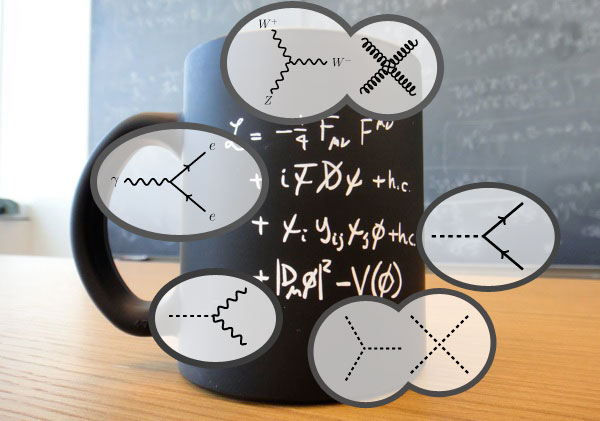
\includegraphics[width=\textwidth]{img/hrnek.jpg}
	\caption{Hrneček ze Švýcarska}
	\label{fig:hrnek}
\end{figure}

\section{Bibliografie}
Citovat je důležité (kruciální) a neméně důležité je citovat správně, a to v~ČR podle normy ČSN ISO 690 a ČSN ISO 690-2.
Důvod, proč ji tak mnoho lidí nedělá, je takový: Jedná se o~pěkně otravnou činnost\cite{citovani}.
To se však dá značně eliminovat použitím vhodného softwaru na správu a export citací.
Jaké máme možnosti?

Přímo českou normou se již dlouhou dobu zabývá projekt Citace.com umožňující zdarma získat toliko potřebné bibliografické záznamy.
Proces zkomfortňování šel až tak daleko, že si (např.) čtenáři registrovaní v~Moravské zemské knihovně (do 19 let vč.
zdarma) mohou nainstalovat do svého Wordu doplněk, který téměř vše zařídí za vás.

Pokud náhodou ještě nemáte a nemůžete mít účet v~Moravské zemské knihovně, nemusíte zoufat, i volně přístupná část nástrojů Citací.com má co nabídnout.
Na webu totiž můžete jednoduše vložit ISBN knihy nebo DOI (\It{Digital object identifier}) článku v~časopise a obratem vám bude vygenerována citace přesně podle normy, kterou můžete jednoduše zkopírovat do Wordu.
Číslování v~textu si však budete muset řešit sami.

Nicméně možnosti nekončí Citacemi.com, existuje celá řada dalších nástrojů (třeba EndNote).
Nebojte se požádat o~pomoc své školitele, sami si nejednou prošli stejným problémem a řešení s~velkou pravděpodobností našli.
Tak proč vynalézat kolo?

\subsection{Užitečné odkazy}
\begin{itemize}
	\item \url{http://www.citace.com}, \url{http://www.mzk.cz/}
	\item \url{http://www.boldis.cz/citace/citace1.pdf}
	\item \url{http://www.boldis.cz/citace/citace2.pdf}
	\item \url{https://sites.google.com/site/novaiso690/}
\end{itemize}

\section{Symboly, zkratky, slovníček}
Zkratky vysvětlujeme již při první zmínce v~textu, při jejich častějším výskytu může být praktické uvést ucelený seznam.
Totéž pak platí pro pojmy, které vysvětlujeme v~poznámce pod čarou\footnote{Poznámku pod čarou vložíme opět z~karty \It{Reference} tlačítkem \It{Vložit pozn.
		pod čarou.}}: pokud jich je mnoho, vysázíme je i samostatně jako slovníček pojmů.

\section{Moudra závěrem}
Uvědomte si, že hlavním výstupem vaší roční činnosti nejsou data nebo zařízení, nýbrž právě odborný text, který má komisi SOČ ukázat, jak jste studované problematice porozuměli, jaký je váš vlastní přínos, jestli dokážete verbálně vystihnout vše podstatné a důležité.
\It{Formální a estetickou úpravou práce sdělujete komisi, jak moc vám záleží na tom, aby pro ně bylo čtení vaší práce příjemným či alespoň snesitelným zážitkem.}

Šablona je míněna jen jakýmsi odrazovým můstkem a nebojte, pořád na vás zbylo docela dost práce.
Bohužel víc, než jsem původně zamýšlel, protože sázení ve Wordu stále není žádný med a byla by jistě škoda ochudit vás o~četné nadávky na nesmyslnost jeho chování.
Všem počítačově zdatným jedincům pak doporučuji naučit se sazbu v~LaTeXu, je to dovednost, která se vám nikdy neztratí.

\begin{figure}[h]
	\centering
	
\includegraphics[width=\textwidth]{img/pulp.jpg}
	\caption{Nejste v~tom sami.}
\end{figure}

Na závěr vám už poradím jen jedno: hledejte inspiraci.
Velmi dobře si pamatuji ten pocit, kdy sedíte nad prázdným dokumentem a přemýšlíte, co vlastně do té SOČky patří.
Kde začít? Co ještě zmínit a co už raději vynechat? Přitom máme všichni díky theses.cz na dosah stovky tisíc závěrečných prací starších kolegů z~vysokých škol.
Najděte si svůj vzor a jeďte podle něj, odborné posudky vedoucích a oponentů vám dokonce řeknou, co je správně a co nikoliv.

\vspace{\baselineskip}
\noindent Vědě zdar!

\vspace{\baselineskip}
\noindent \B{Roman Beránek} \\
\url{ischemy@gmail.com}

\chapter{Slovo Jarka}
Trochu bych nesouhlasil s~Romanem ohledně „hlavního výstupu vaší roční činnosti“ a také se zdroji, odkud je vhodné čerpat inspiraci.

Rád bych tato dvě témata na závěr trochu rozebral a zároveň přidal pár slov o~prezentacích, které by měly tvořit podstatnou část vaší práce.

\section{Hlavní výstup vaší roční činnosti}
U~některých oborů možná platí, že hlavním výstupem vaší roční činnosti nejsou data nebo zařízení, nýbrž právě odborný text.
Ovšem z~vlastní zkušenosti mohu říct, že pokud předvedete funkční výtvor (a to ať už softwarový balík pro vývoj a řízení aplikací s~mikročipy, výukový webový portál, univerzální ovládací pult, nebo regulovatelný napájecí zdroj) budete mít na 90 \% větší úspěch než čistě teoretická práce.

Samozřejmě pokud někdo vyvrátí teorii relativity nebo vymyslí novou a lepší periodickou tabulku prvků, bude mít pravděpodobně lepší pozici než vy.
Proto ale musí být vaše práce co možná nejlepší.

Pokud donesete výrobek, který je inovativní, nadčasový, velmi nápaditý a případně vyrobitelný nebo dokonce komerčně prodatelný, a dokážete ho při prezentaci prodat (o~důležitosti prezentace více informací níže), většina porotců vám promine i formální nedostatky a krátký rozsah práce, protože jste jim to předvedli naživo (minimálně toto platí v~rámci oboru strojírenství, elektra a informatiky a podle mě i fyziky, učebních pomůcek atd.)

Kdybych to vzal do extrému, tak práce, která nemá text, ale je velmi zajímavá pro svůj výrobek (zařízení), může klidně vyhrát celostátní kolo SOČ.
Ovšem když přijdu s~textem, kde tento výrobek dokonale popisuji, ale nedovezu, nepředvedu, neukáži, že je funkční, tak jsem na tom hůř než v~prvním případě.

Toto jsou ovšem specifika spíše techničtějších oborů (s~kterými mám zkušenost) a je možné, že v~přírodních vědách (jako chemie, matika, biologie) má spíše Roman pravdu, ale nejsem si tím úplně jistý.
Zvažte sami~:-)

\section{Kde čerpat inspiraci}
Roman jako inspiraci doporučoval theses.cz, ovšem já bych vás spíše odkázal na archiv SOČ (\url{http://soc.nidm.cz/archiv}) a to ze tří důvodů:

\begin{enumerate}[label=\alph*)]
	\item Uvidíte styl a způsob zpracování úspěšných prací SOČ, které vytvořili studenti ve vašem věku a které se porotcům líbily.
	\item Nemusíte se probírat stovkami tisíc závěrečných prací, ale jednoduše si vyberete váš obor a projdete několik nejlepších prací za posledních pár let.
	\item Styl bakalářských a diplomových prací se od SOČek trochu liší a občas je lepší se držet zaběhnutých pravidel SOČ.
\end{enumerate}
Samozřejmě si můžete projít i několik vysokoškolských prací a třeba v~nich najdete i lepší inspiraci.

Jinak nad samostatným formátováním (či některými detaily) neztrácejte mnoho času, protože vám pravděpodobně schází ještě podstatnější věci.
A~také platí, že co porotce/obor, to jiný názor na některé detaily formátování SOČek :-)

\section{Prezentace}
Sebelepší práce bez dobré prezentace je prakticky k~ničemu.
Porotci v~nižších kolech (okresních i krajských) nemají často čas prostudovat si text práce předem.
Tudíž jej občas vidí poprvé, až když danou práci prezentujete.

Pokud budete mít dobrou prezentaci, ve které svoji práci dobře prodáte – ukážete, co jste dělali, jak jste to dělali, co je vaše práce, ale hlavně co je tak unikátního na vaší práci a proč zrovna vy byste měli vyhrát), tak máte z~poloviny vyhráno.
Prezentace tvoří klidně i polovinu hodnocení vaší práce.
Nebo víc.

Proto je podle mě důležité věnovat minimálně stejné množství času přípravě prezentace jako textu.
Pokud postoupíte do dalšího kola, máte většinou možnost si svou práci vzít a do týdne ji upravit/doladit.
Samozřejmě že pokud budete mít perfektní text hned do prvního kola SOČ, budete mít výhodu vůči ostatním a lepší startovací pozici do dalších kol, ale v~případě nedostatku času (což většinou bývá) je vhodnější rozdělit si čas mezi tvorbu textů, prezentace a případně samostatného výrobku.

Samozřejmě se nebojte inspirovat u~svých kolegů z~minulých let například na serveru YouTuBe (hledejte pod „CP SOČ 2013“ a „SOČ 2013 – Brno – krajské kolo“).

O~prezentacích se toho dá samozřejmě napsat mnoho, ale to si necháme třeba na příště ;-)

\vspace{\baselineskip}
\noindent SOČce zdar!

\vspace{\baselineskip}
\noindent \B{Jarek Páral}\\
\url{paral.jarek@gmail.com}

\chapter{Ještě slovo Lucie}
Pokud si nebudete jistí typografií nebo pravopisem, konzultujte vynikající Internetovou jazykovou příručku.
Píšou ji autoři z~Ústavu pro jazyk český a mezi množstvím balastu na Internetu jí můžete věřit.
Stačí většinou zadat do Google problémové slovo nebo znak spolu s~heslem „ujc“ a víte, na čem jste.

Doufám, že jsme vám pomohli a zpříjemnili práci na vaší SOČce a že shledáte šablonu přínosnou.
Za podněty a reakce budeme všichni tři rádi.

\vspace{\baselineskip}
\noindent Ať to jde!

\vspace{\baselineskip}
\noindent \B{Lucie Vaškeová} \\
\url{lucie.vaskeova@jcmm.cz}

\newpage
\chapter*{Závěr}
\addcontentsline{toc}{section}{Závěr}

Závěrečná kapitola obsahuje zhodnocení dosažených výsledků se zvlášť vyznačeným vlastním přínosem studenta.
Povinně se zde objeví i zhodnocení z~pohledu dalšího vývoje projektu, student uvede náměty vycházející ze zkušeností s~řešeným projektem a uvede rovněž návaznosti na právě dokončené projekty.